\documentclass[11pt,a4paper]{article}
\usepackage[utf8]{inputenc}
\usepackage[T1]{fontenc}
\usepackage{tgpagella}
\usepackage[spanish]{babel}
\usepackage{geometry}
\usepackage{graphicx}
\usepackage{booktabs}
\usepackage{array}
\usepackage{xcolor}
\usepackage{titlesec}
\usepackage{fancyhdr}
\usepackage[parfill]{parskip}
\usepackage[expansion=false]{microtype}
\usepackage{hyperref}
\usepackage{setspace}
\usepackage{needspace}

\geometry{top=3.0cm,bottom=3.0cm,left=3.5cm,right=3.5cm}
\setlength{\parskip}{0.65em}
\setlength{\parindent}{0em}

\definecolor{azulai}{RGB}{30,80,140}
\definecolor{doradoai}{RGB}{140,90,0}
\definecolor{grisai}{RGB}{70,70,70}

\titleformat{\section}{\Large\bfseries\color{azulai}}{}{0em}{}[{\color{azulai}\titlerule[0.5pt]\nopagebreak[4]}]
\titlespacing*{\section}{0pt}{1.8em}{0.8em}
\titleformat{\subsection}{\large\bfseries\color{doradoai}}{}{0em}{}[{\nopagebreak[4]}]
\titlespacing*{\subsection}{0pt}{1.4em}{0.5em}
\titleformat{\subsubsection}{\normalsize\bfseries\color{grisai}}{}{0em}{}[{\nopagebreak[4]}]
\titlespacing*{\subsubsection}{0pt}{1.0em}{0.3em}

\pagestyle{fancy}\fancyhf{}
\rhead{\textcolor{grisai}{\small Urko — Arquitectura Interna}}
\lhead{\textcolor{grisai}{\small Carta Natal Completa}}
\cfoot{\textcolor{grisai}{\small\thepage}}
\renewcommand{\headrulewidth}{0.3pt}

\hypersetup{colorlinks=true,linkcolor=azulai,urlcolor=azulai}
\setstretch{1.45}
\tolerance=1500
\emergencystretch=4em

\begin{document}

% ── Portada ──────────────────────────────────────────────────────────────────
\begin{titlepage}
  \centering
  \vspace*{1.5cm}
  {\Huge\bfseries\color{azulai} Carta Natal Completa}\\[0.5cm]
  {\large\color{grisai} Arquitectura Interna}\\[0.3cm]
  {\small\itshape\color{grisai} Un método para sostener cuerpo, energía y vida con coherencia}\\[2cm]
  {\huge\color{doradoai} Urko}\\[1.5cm]
  {\Large 11/12/2015 \quad 22:47}\\[0.3cm]
  {\Large Pamplona, España}\\[0.3cm]
  {\normalsize Lat: 42.8157° \quad Lon: -1.6522° \quad UTC+01:00}\\[0.3cm]
  {\normalsize Ascendente: Leo 25°29' \quad
    MC: Tauro 17°51'}\\[2.5cm]
  \vfill
  {\small Generado el 09/05/2026}
\end{titlepage}

\tableofcontents
\newpage

% ── Rueda ─────────────────────────────────────────────────────────────────────
\section{Carta Natal}
\begin{figure}[h!]
  \centering
  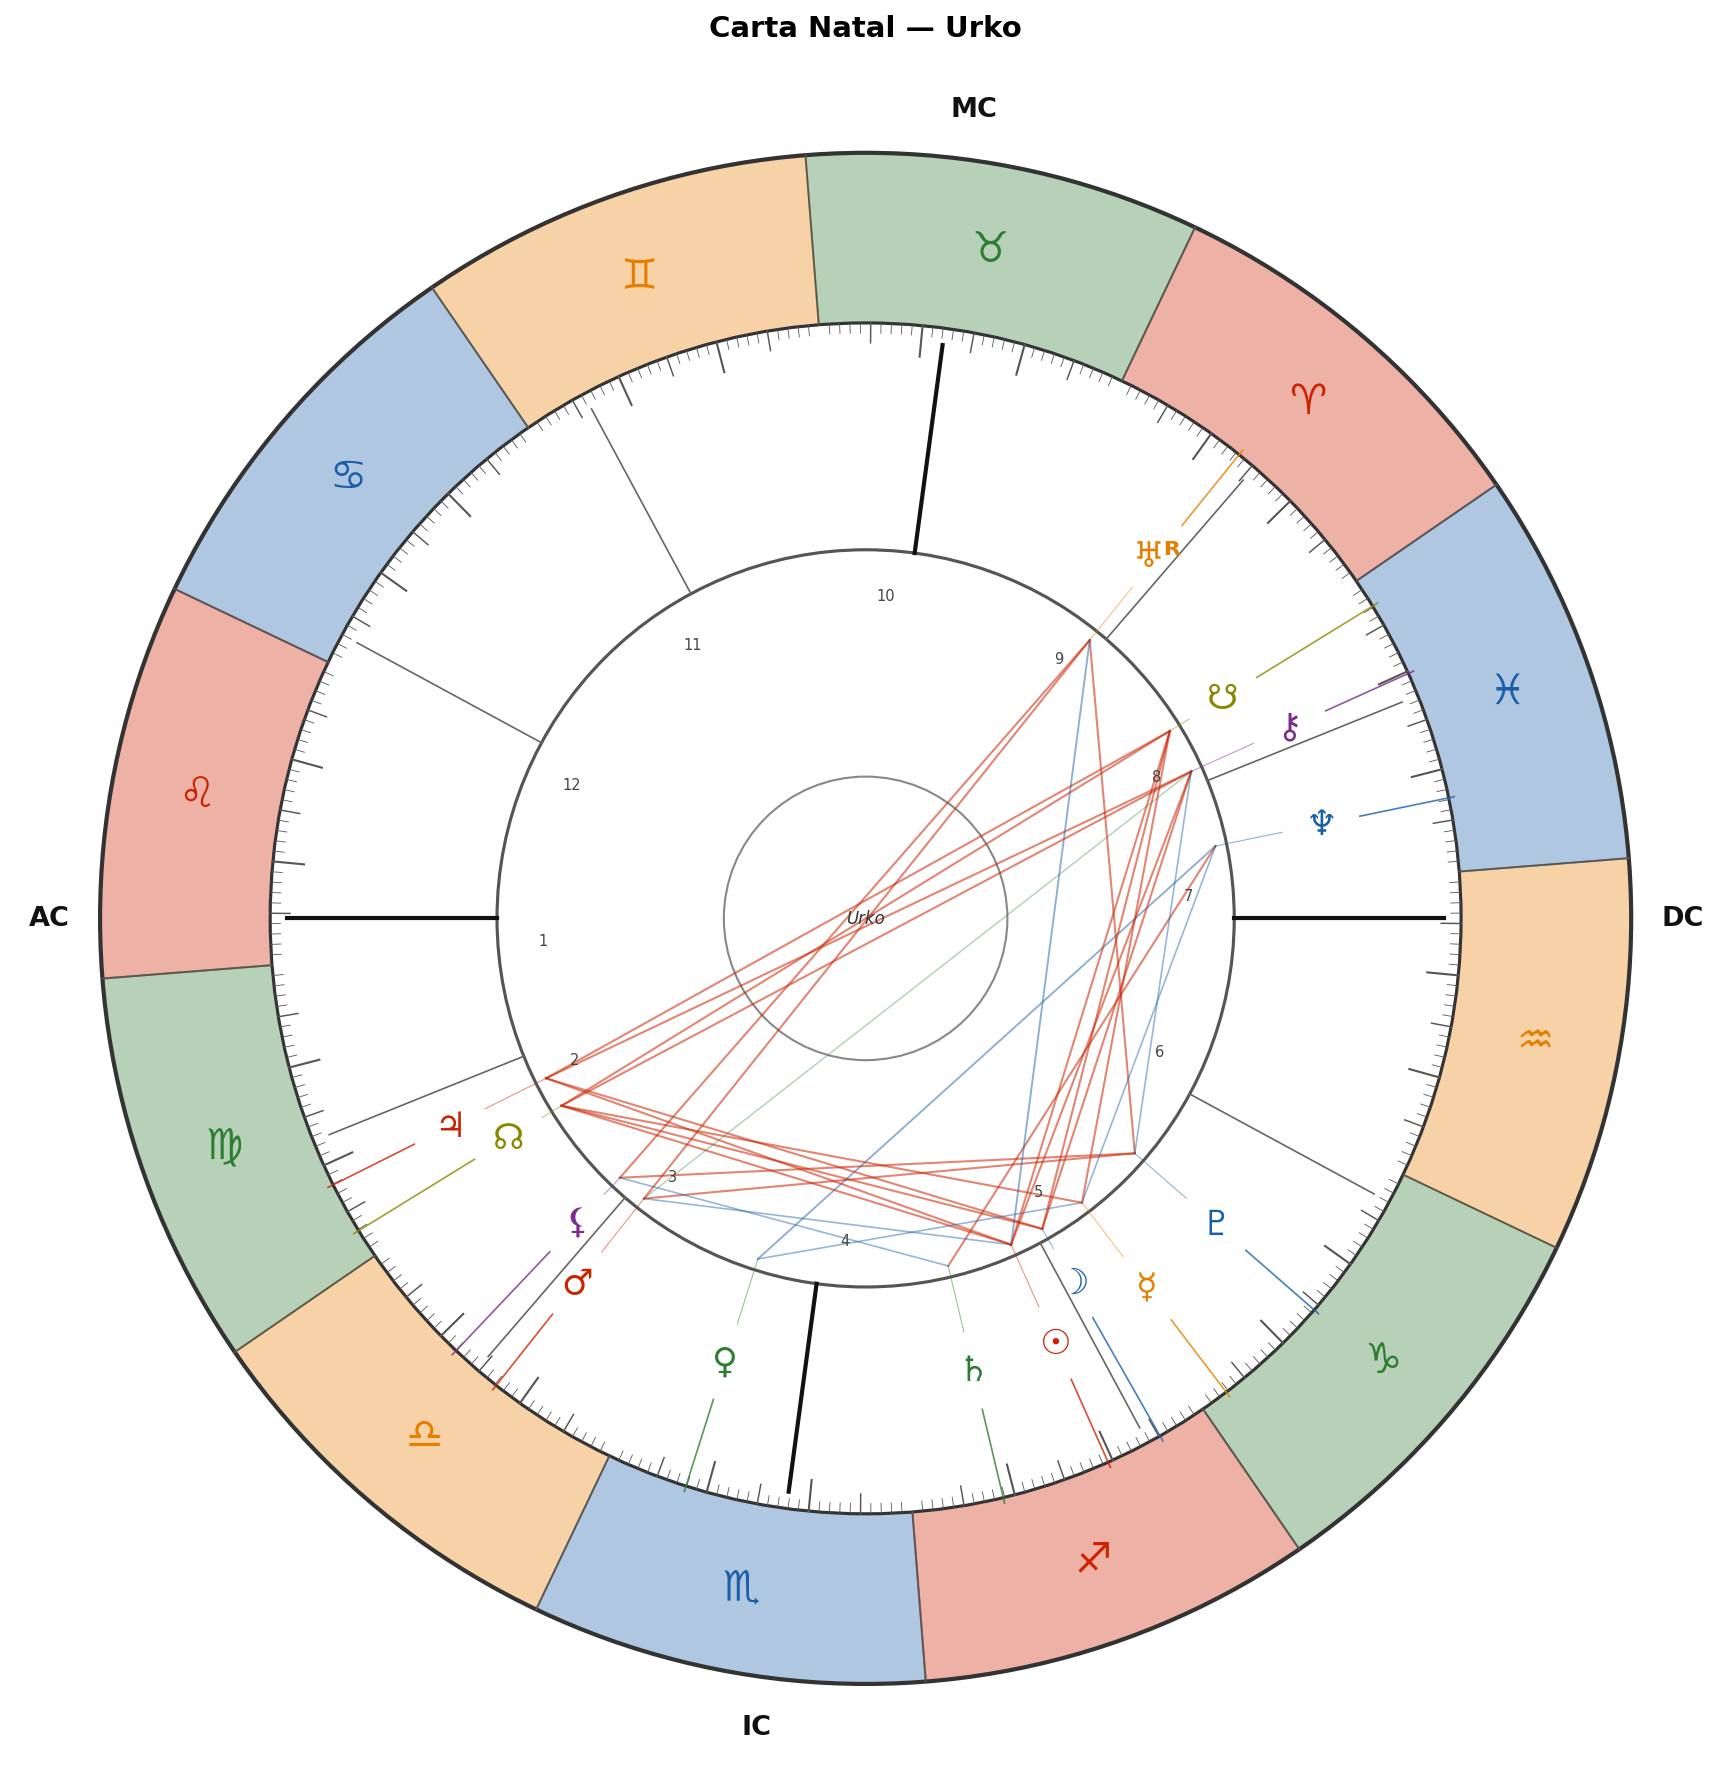
\includegraphics[width=0.90\textwidth]{Urko_AI_rueda.png}
  \caption{Carta natal de Urko — 11/12/2015 22:47 — Pamplona, España}
\end{figure}

\newpage

% ── Tabla de posiciones ───────────────────────────────────────────────────────
\section{Posiciones Planetarias}

\begin{center}
\begin{tabular}{llrrlll}
  \toprule
  \textbf{Planeta} & \textbf{Signo} & \textbf{Grado} & \textbf{Casa} &
  \textbf{Elemento} & \textbf{R} \\
  \midrule
  Sol & Sagitario & 19°32' & 4 & Fuego &  \\
  Luna & Sagitario & 25°07' & 5 & Fuego &  \\
  Mercurio & Capricornio & 2°46' & 5 & Tierra &  \\
  Venus & Escorpio & 7°56' & 3 & Agua &  \\
  Marte & Libra & 17°09' & 3 & Aire &  \\
  Júpiter & Virgo & 22°05' & 2 & Tierra &  \\
  Saturno & Sagitario & 8°51' & 4 & Fuego &  \\
  Urano & Aries & 16°39' & 9 & Fuego & R \\
  Neptuno & Piscis & 7°10' & 7 & Agua &  \\
  Plutón & Capricornio & 14°22' & 5 & Tierra &  \\
  Quirón & Piscis & 19°47' & 8 & Agua &  \\
  Lilith & Libra & 12°02' & 2 & Aire &  \\
  Nodo Norte & Virgo & 27°07' & 2 & Tierra &  \\
  Nodo Sur & Piscis & 27°07' & 8 & Agua &  \\
  \bottomrule
\end{tabular}
\end{center}

\vspace{0.5cm}
\begin{itemize}
  \item \textbf{Ascendente:} Leo 25°29'
  \item \textbf{Medio Cielo:} Tauro 17°51'
\end{itemize}

\newpage

% ── Interpretación ────────────────────────────────────────────────────────────
\section{Interpretación — Arquitectura Interna}

\begin{center}
{\small\itshape
No se trata de definirte. Se trata de observar cómo se organiza tu energía,\
dónde puedes perder equilibrio y qué apoyos te ayudan a sostenerte.
}
\end{center}

\vspace{0.5cm}

\subsection{1. Visión General}

Tu carta muestra la siguiente distribución de elementos: Fuego 9, Tierra 3.5, Aire 1.5, Agua 2.5. Fuego (vitalidad, iniciativa, necesidad de sentido y movimiento hacia la acción): ahí está el peso de tu carta. Es el registro desde el que tu energía se activa con más fluidez y sin esfuerzo consciente. Aire (desapego, análisis, pensamiento relacional y capacidad de perspectiva) está poco representado en tu carta. Ese territorio puede pedirte un esfuerzo consciente, especialmente cuando la presión sube. La mayoría de tus planetas están en signos mutables: hay facilidad para adaptarte, cambiar y responder a lo que ocurre alrededor. Sueles moverte bien cuando las situaciones evolucionan o requieren flexibilidad. La dificultad aparece cuando todo cambia al mismo tiempo y cuesta mantener una dirección estable durante suficiente tiempo. Tu Medio Cielo en Tauro: La constancia, la paciencia y la construcción de algo sólido con el tiempo. Tu presencia pública suele percibirse como estable y fiable.

\subsection{2. Ejes Principales}

\subsubsection*{Sol en Sagitario — Casa 4}
Tu Sol en Sagitario necesita sentir que lo que haces tiene dirección y sentido para ti. Funcionas mejor cuando hay movimiento, aprendizaje o sensación de expansión. La capacidad de entusiasmarte y abrir perspectivas suele aparecer de forma natural. El riesgo aparece cuando la necesidad de avanzar hace difícil detenerte en lo cotidiano o sostener procesos lentos. En Casa 4, necesitas una base emocional estable desde la que moverte. La sensación de hogar, intimidad y protección tiene mucho peso en cómo te desarrollas. Sueles necesitar espacios donde bajar la guardia y sentir que no tienes que sostener nada hacia afuera constantemente. Cuando esa base falta, el desgaste aparece aunque externamente todo parezca funcionar.

\subsubsection*{Luna en Sagitario — Casa 5}
Tu Luna en Sagitario necesita movimiento, perspectiva y sentido. Cuando algo te afecta, te ayuda entender para qué sirve, hacia dónde te lleva o qué puedes hacer con ello. Si no encuentras una salida, el estado emocional puede convertirse en inquietud, impaciencia o necesidad de cambiar de escenario. El movimiento, el cambio de perspectiva y la sensación de amplitud te ayudan a recuperar estabilidad. En Casa 5, tu seguridad emocional se activa a través de la expresión creativa, el juego y el amor. Necesitas que tu vida emocional tenga un componente de disfrute y de expresión auténtica.

\subsubsection*{Ascendente Leo}
Tu Ascendente en Leo hace que te muestres al mundo con calidez, presencia y una orientación natural a ocupar el espacio con seguridad. Entras al entorno con una energía que otros notan. La necesidad de expresarte y ocupar espacio suele percibirse desde el primer contacto. Su regente es el Sol, en Sagitario y Casa 4. El Ascendente toma el tono de Sagitario: expansiva, entusiasta y orientada a ampliar horizontes. Esa energía opera principalmente desde el hogar, la intimidad y la necesidad de una base emocional estable.


\subsection{3. Organización de la Energía}

Tu Mercurio en Capricornio piensa de forma práctica, ordenada y orientada a resultados. Necesitas estructura, claridad y pasos concretos para organizar bien una idea. El riesgo aparece cuando la mente se vuelve demasiado rígida o tarda en permitirse probar algo nuevo. En Casa 5, la mente necesita creatividad, expresión y cierta libertad para funcionar bien. Piensas mejor cuando hay entusiasmo, juego o posibilidad de poner algo personal en lo que haces. Tu Venus en Escorpio se vincula con intensidad y necesidad de confianza real. No te alimentan los vínculos superficiales cuando algo importa de verdad. El riesgo aparece cuando el miedo a perder o a quedar expuesto lleva a controlar más de lo necesario. En Casa 3, el afecto fluye especialmente a través de la conversación, la cercanía y el intercambio cotidiano. La comunicación tiene mucho peso en cómo se construyen tus relaciones. Tu Marte en Libra actúa mejor cuando hay acuerdo, colaboración o una dirección compartida. Antes de moverte, sueles tener en cuenta a la otra persona. El riesgo aparece cuando esperar equilibrio o aprobación retrasa una acción que ya necesita hacerse. En Casa 3, la energía se expresa mucho a través de la palabra, las ideas y el movimiento cotidiano. El debate, el intercambio o la necesidad de responder rápido pueden activarse fácilmente.

\subsection{4. Estructura y Tensión}

\subsubsection*{Concentración de energía}

Hay una concentración notable en Casa 5: Luna, Mercurio y Plutón. Cuando varios planetas ocupan la misma casa, esa área absorbe buena parte de la actividad vital. En esta carta, el foco de la creatividad, el disfrute y la expresión personal funciona como núcleo central: ahí se acumula la presión, la demanda es mayor y también hay más recursos disponibles para operar. No es necesariamente un conflicto, pero sí un punto de alta intensidad sostenida.

También hay una concentración significativa en Casa 2: Júpiter, Nodo Norte y Lilith. En este caso, el foco se desplaza hacia los recursos, la estabilidad y el valor propio. Es un ámbito donde la exigencia aumenta, donde se concentra parte de la presión y donde también existe capacidad real de sostener procesos importantes. Tampoco es en sí un problema, pero sí un área de intensidad mantenida.



Los aspectos aparecen organizados en dos niveles. Los aspectos exactos (orbe igual o menor a 1°) suelen sentirse de forma más inmediata y constante en la vida cotidiana. Los aspectos estructurales tienen un orbe más amplio, pero siguen describiendo dinámicas importantes que se repiten a lo largo de la vida.



\Needspace{8\baselineskip}
\subsubsection*{Aspectos exactos}
No aparecen aspectos exactos especialmente fuertes dentro del orbe definido para esta lectura. Eso no significa ausencia de tensión o profundidad, sino que gran parte de las dinámicas importantes de la carta se construyen de forma más amplia y progresiva. En este caso, cobran más importancia los aspectos estructurales y la combinación general de posiciones.

\Needspace{8\baselineskip}
\subsubsection*{Aspectos estructurales}
\Needspace{7\baselineskip}
\subsubsection*{Sol (Casa 4) cuadratura Júpiter (Casa 2) --- orbe 2.55\textdegree}
La cuadratura Sol-Júpiter puede llevarte a ampliar más de lo que puedes sostener. Hay entusiasmo, visión y capacidad de crecimiento, pero también tendencia a asumir demasiado o confiar en que podrás con todo. El límite no viene a apagar la expansión, sino a darle una forma que no te desgaste.



\subsection{5. Sostén y Equilibrio}

Tu Quirón en Piscis, Casa 8, señala una zona sensible relacionada con los límites, la sensibilidad y la dificultad para diferenciar lo propio de lo ajeno. Puede que te haya costado sostener claridad cuando el entorno emocional era muy intenso. Esto suele notarse especialmente en la intimidad, las pérdidas y las situaciones emocionalmente intensas. No significa que tengas límites en ese terreno, pero sí que probablemente necesites más tiempo, cuidado o consciencia para sentir estabilidad ahí.

\vspace{0.3cm}
Tu Nodo Sur en Piscis, Casa 8, muestra una tendencia a moverte desde la falta de límites claros, la adaptación excesiva o la tendencia a perderte en el entorno, especialmente en la intimidad y las situaciones emocionalmente intensas. Suele ser una forma de funcionar conocida o automática para ti. Tu Nodo Norte en Virgo, Casa 2, señala la necesidad de desarrollar desarrollar orden, presencia en lo cotidiano y capacidad de concretar, especialmente en el valor propio y la estabilidad material o emocional. No se trata de rechazar lo anterior, sino de ampliar tu forma habitual de responder.

\vspace{0.3cm}


\subsection{6. Orientación}

\subsubsection*{Qué observar}
Tu Ascendente en Leo describe la forma en que otras personas suelen percibirte al principio. Eso no siempre coincide con cómo vives las cosas internamente o con las tensiones más importantes de tu carta. Cuando hay demasiada distancia entre lo que muestras y lo que realmente te ocurre, aparece desgaste.

\subsubsection*{Qué puede desestabilizar}
Hay ciertas tensiones en tu carta que pueden activarse con bastante fuerza: Nodo Norte-Nodo Sur, Sol-Quirón, Marte-Urano. Cuando varias coinciden al mismo tiempo, puede aparecer sensación de saturación, reacción excesiva o dificultad para mantener claridad.

\subsubsection*{Qué estructura y sostiene}
Tu Sol en Sagitario, Casa 4, muestra un terreno importante de estabilidad para ti. Cuando tu forma de actuar está alineada con lo que realmente valoras, suele aparecer más claridad y menos dispersión.

\subsubsection*{Orientación práctica}
Una orientación práctica: cuando todo se activa demasiado, no intentes resolverlo todo desde la cabeza. Empieza por algo pequeño y concreto que te devuelva presencia: caminar, ordenar una parte de tu espacio, cocinar, respirar con calma o hacer algo físico y sencillo. Muchas veces el cuerpo recupera claridad antes que la mente.

\vspace{1cm}
\begin{center}
{\small\itshape\color{grisai}
La astrología se usa aquí como lenguaje simbólico de observación, no como una definición de quién eres.\\
Esta interpretación es tu mapa de posibilidades, no tu destino fijo.
}
\end{center}

\end{document}
